\begin{table*}[t]
\label{tab:experiments}
\caption{Accumulated rewards split by origin per experiment. Evaluation were done after every epoch and the best result is shown.}
\vskip 0.15in
\begin{center}
\begin{small}
\begin{sc}
\begin{tabular}{lcccccr}
\toprule
Experiment & Algorithm & ESS & FDR & TCL & Discomfort & Total \\
\midrule
\multirow{4}{*}{Full Environment} 
    & Idle      & 0.00   & -3173.56 & \textbf{-9887.61}  & -5912.63 & -18973.80 \\
    & Threshold & \textbf{633.24} & \textbf{-3071.35} & -9957.07  & -5557.23 & -17952.41 \\
    & PPO       & 0.00   & -3233.98 & -10825.89 & \textbf{-788.15} & \textbf{-14847.02} \\
    & SAC       & 60.24  & -3087.39 & -14692.60 & -1637.00 & -19356.75 \\
\midrule
\multirow{4}{*}{Hypothesis 1}
    & Idle      & 0.00   & -3173.56 & \textbf{-9887.61} & -5912.63 & -18973.80 \\
    & Threshold & \textbf{633.24} & \textbf{-3068.56} & -9957.07 & -5557.23 & -17949.62 \\
    & PPO       & 0.00   & -3151.34 & -11058.75& \textbf{-531.89} & \textbf{-14741.98} \\
    & SAC       & -40.18 & -3192.11 & -14329.95 & -1258.60 & -19820.84 \\
\midrule
\multirow{4}{*}{Hypothesis 2} 
    & Idle      & 0.00   & -3173.56 & \textbf{-9887.61} & -5912.63 & -18973.80 \\
    & Threshold & \textbf{633.24} & -3068.56 & -9957.07 & -5557.23 & -17949.62 \\
    & PPO       & 488.58 & -3035.30 & -10755.65 & \textbf{-3152.03} & \textbf{-14454.40} \\
    & SAC       & 157.94 & \textbf{-2969.78} & -10114.51 & -4906.66 & -17832.01 \\
\midrule
\multirow{4}{*}{Hypothesis 3} 
    & Idle      & 0.00   & -3173.56 & \textbf{-9887.61} & -5912.63 & -18973.80 \\
    & Threshold & 633.24 & -3068.56 & -9957.07 & \textbf{-5557.23} & \textbf{-17949.62} \\
    & PPO       & \textbf{650.49} & -3170.04 & -10512.15 & -5913.87 & -18945.57 \\
    & SAC       & 599.65 & \textbf{-2969.36} & -52971.76 & -13164.96 & -67506.43 \\
\bottomrule
\end{tabular}
\end{sc}
\end{small}
\end{center}
\vskip -0.1in
\end{table*}

As non-learning baselines an idle policy, which would always return zero actions, whose cumulative reward in the first episode is shown in \cref{fig:reward_idle}, and a thresholding policy, see \cref{sec:thresholding_baseline}, were implemented.

\begin{figure}[H]
    \centering
    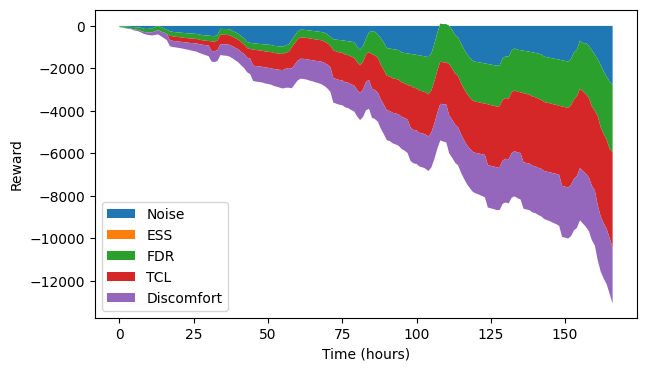
\includegraphics[width=0.45\textwidth]{figures/idle_reward.png}
    \caption{Cumulative reward for the idle policy.}
    \label{fig:reward_idle}
\end{figure}

As learning agents, Soft Actor Critic (SAC) \cite{Haarnoja.04.01.2018} and Proximal Policy Optimization (PPO) \cite{Schulman.20.07.2017} were chosen. Both implementations were taken from stable baselines 3 \cite{AntoninRaffin.2021}, for details see \cref{sec:sac} and \cref{sec:ppo}.
\par
To allow for differentiation on which sub-tasks the agent performs well, the reward was split by the component of origin, as in \cref{sec:split_reward}. 
\par
The results of all experiments are shown in \cref{tab:experiments}. Since the initial task did not yield reward convergence surpassing the baselines, as shown in \cref{fig:training_curve}, three hypothesis with accompanying modifications to the environment were tested. The changes were cumulative and further details can be found in \cref{sec:training_procedure}.
\begin{figure}[H]
    \centering
    \setlength{\abovecaptionskip}{0pt}
    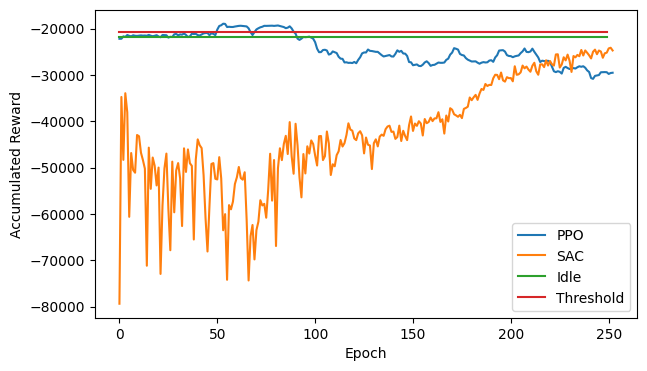
\includegraphics[width=0.45\textwidth]{figures/training_curve.png}
    \caption{Training curve of the Full Environment.}
    \label{fig:training_curve}
\end{figure}


\subsection{Scheduling, Stochasticity, and Dimensionality}
The challenge of learning in the FDR sub-task is innate in scheduling \cite{Zhang.23.10.2020} but is further complicated by the stochastic control. Furthermore, it bloats the dimensionality of the spaces with decreasing resolution, since the time window was always 24 hours.
\par
To ease those challenges the control was changed to deterministic, and scalar and the observation included only the sum of the time window. These changes are equivalent to the assumption that the optimal policy is invariant to $U_e$ as long as the sum is maintained and that $\beta = \infty$.
\par
The modified task only showed improvements for minutely resolution, which suggests that high dimensionality is a problem. However, since convergence was still absent, the inefficiency of the other changes could not be concluded.


\subsection{Hard Exploration}
The environment still provides a vast exploration space, due to the continuity of the spaces and the length of the episodes. Moreover, there is significant noise from the RSA and fixed demand on the reward. Moreover, a lot of observables are only relevant for estimating the future carbon intensity. 
\par
To address this the minutely resolution was omitted, the action space for PPO was discretised, the fixed demand and RSA were removed from the observables and reward calculation, and the agents were trained separately for every sub-task. Lastly, the replay buffer for SAC was initialized with transitions of the threshold algorithm, providing a warm start \cite{Wang.20.06.2023}.
\par
The result indicated, that the discretisation aided PPO in learning the ESS but hindered in the TCL sub-task, hinting too coarse discretisation. SAC did not benefit from the warm start after a few epochs. 


\subsection{Delayed or Deceptive reward}
Another challenge of the setting is the reward structure for charging the ESS, expediting the FDR and heating or cooling the TCL. The rewards of those actions always occur delayed and only if the respective counter action is performed at a higher carbon intensity, which can be problematic \cite{Sutton.1984}. Moreover, the rewards might even be deceptive, since those actions are necessary for an effective policy but only ever receive negative reward.
\par
To test the hypothesis, the reward was transferred to an accumulating observable and only actuated in the terminal state, which should encourage the agent to evaluate the entire trajectory of an episode holistically.
\par 
Since the task was hardened by this change performance was expectedly decreased for TCL and FDR. However, the ESS sub-task showed signs of improvements but no convergence within the 250 epochs.